\documentclass[12pt]{article}
\usepackage[table]{xcolor}
\usepackage[shortlabels]{enumitem}
\usepackage{tabularx,xltabular}
\usepackage{graphicx}
\usepackage{hyperref}
\usepackage{verbatim}
\usepackage{geometry}
\usepackage{ulem}
\usepackage[official]{eurosym}
\usepackage{tikz}
\usetikzlibrary{arrows,backgrounds,calc,decorations.markings,patterns,3d,positioning,fit,angles, quotes}
\usepackage{pgfplots}
\pgfplotsset{compat = newest}
\usetikzlibrary{fit}
\newcommand\addvmargin[1]{
\usetikzlibrary{arrows}
\node[fit=(current bounding box),inner ysep=#1,inner xsep=0]{};}
\usepackage{cancel}
\usepackage{fontspec}
\usepackage{array}  
\geometry{a4paper, top=2cm, left=2cm, right=2cm, bottom=2cm, headsep=1cm}
\usepackage{tabu}
\usepackage{pst-node}
\usepackage{colortbl}
\usepackage{array}
\usepackage{german}
\setlength\parindent{0pt}
\newcolumntype{?}{!{\vrule width 1pt}}
\usepackage{makecell}
\renewcommand{\arraystretch}{2.5}
\usepackage{pbox}
\usepackage{amssymb}
\usepackage{amsmath}
\usepackage{booktabs}
\newcolumntype{L}[1]{>{\raggedright\let\newline\\\arraybackslash\hspace{0pt}}m{#1}}
\newcolumntype{C}[1]{>{\centering\let\newline\\\arraybackslash\hspace{0pt}}m{#1}}
\newcolumntype{R}[1]{>{\raggedleft\let\newline\\\arraybackslash\hspace{0pt}}m{#1}}
\begin{document}
\rightline{Datum: 08.12.2023}
\centerline{{\Large Tägliche Übungen}} 
\vspace{1cm}
\noindent \\


\begin{xltabular}{\textwidth}{|C{0.75cm}|X|C{0.75cm}|X|}
\arrayrulecolor{black}\hline
a)&\pbox{5cm}{
Berechne die Fläche von
\tikzstyle{background grid}=[draw, black!15,step=.5cm]
\noindent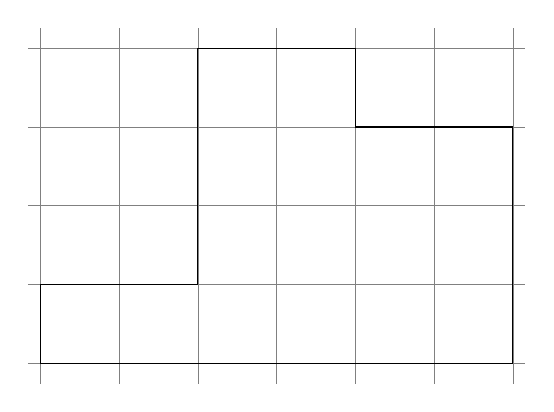
\begin{tikzpicture}[show background grid]
\draw[black] (0cm,0cm) -- (0cm,1cm);
\draw[black] (0cm,0cm) -- (0cm,1cm);
\draw[black] (0cm,1cm) -- (2cm,1cm);
\draw[black] (2cm,0.0cm) -- (0cm,0.0cm);
\draw[black] (2cm,1cm) -- (2cm,4cm);
\draw[black] (2cm,1cm) -- (2cm,4cm);
\draw[black] (2cm,4cm) -- (4cm,4cm);
\draw[black] (4cm,0.0cm) -- (2cm,0.0cm);
\draw[black] (4cm,4cm) -- (4cm,3cm);
\draw[black] (4cm,4cm) -- (4cm,3cm);
\draw[black] (4cm,3cm) -- (6cm,3cm);
\draw[black] (6cm,0.0cm) -- (4cm,0.0cm);
\draw[black] (6cm,3cm) -- (6cm,0.0cm);
\addvmargin{1mm}
\end{tikzpicture}
}
&
b)&\pbox{5cm}{
Berechne die Fläche von
\tikzstyle{background grid}=[draw, black!15,step=.5cm]
\noindent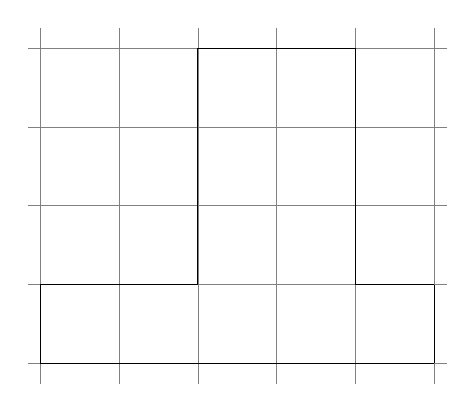
\begin{tikzpicture}[show background grid]
\draw[black] (0cm,0cm) -- (0cm,1cm);
\draw[black] (0cm,0cm) -- (0cm,1cm);
\draw[black] (0cm,1cm) -- (2cm,1cm);
\draw[black] (2cm,0.0cm) -- (0cm,0.0cm);
\draw[black] (2cm,1cm) -- (2cm,4cm);
\draw[black] (2cm,1cm) -- (2cm,4cm);
\draw[black] (2cm,4cm) -- (4cm,4cm);
\draw[black] (4cm,0.0cm) -- (2cm,0.0cm);
\draw[black] (4cm,4cm) -- (4cm,1cm);
\draw[black] (4cm,4cm) -- (4cm,1cm);
\draw[black] (4cm,1cm) -- (5cm,1cm);
\draw[black] (5cm,0.0cm) -- (4cm,0.0cm);
\draw[black] (5cm,1cm) -- (5cm,0.0cm);
\addvmargin{1mm}
\end{tikzpicture}
}
\\\hline
c)&\pbox{5cm}{
Berechne die Fläche von
\tikzstyle{background grid}=[draw, black!15,step=.5cm]
\noindent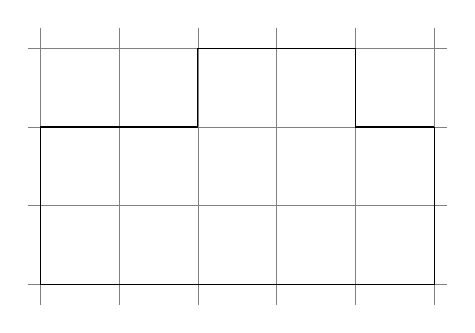
\begin{tikzpicture}[show background grid]
\draw[black] (0cm,0cm) -- (0cm,2cm);
\draw[black] (0cm,0cm) -- (0cm,2cm);
\draw[black] (0cm,2cm) -- (2cm,2cm);
\draw[black] (2cm,0.0cm) -- (0cm,0.0cm);
\draw[black] (2cm,2cm) -- (2cm,3cm);
\draw[black] (2cm,2cm) -- (2cm,3cm);
\draw[black] (2cm,3cm) -- (4cm,3cm);
\draw[black] (4cm,0.0cm) -- (2cm,0.0cm);
\draw[black] (4cm,3cm) -- (4cm,2cm);
\draw[black] (4cm,3cm) -- (4cm,2cm);
\draw[black] (4cm,2cm) -- (5cm,2cm);
\draw[black] (5cm,0.0cm) -- (4cm,0.0cm);
\draw[black] (5cm,2cm) -- (5cm,0.0cm);
\addvmargin{1mm}
\end{tikzpicture}
}
&
d)&\pbox{5cm}{
Berechne die Fläche von
\tikzstyle{background grid}=[draw, black!15,step=.5cm]
\noindent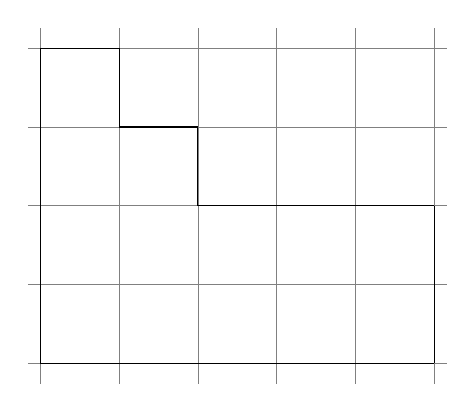
\begin{tikzpicture}[show background grid]
\draw[black] (0cm,0cm) -- (0cm,4cm);
\draw[black] (0cm,0cm) -- (0cm,4cm);
\draw[black] (0cm,4cm) -- (1cm,4cm);
\draw[black] (1cm,0.0cm) -- (0cm,0.0cm);
\draw[black] (1cm,4cm) -- (1cm,3cm);
\draw[black] (1cm,4cm) -- (1cm,3cm);
\draw[black] (1cm,3cm) -- (2cm,3cm);
\draw[black] (2cm,0.0cm) -- (1cm,0.0cm);
\draw[black] (2cm,3cm) -- (2cm,2cm);
\draw[black] (2cm,3cm) -- (2cm,2cm);
\draw[black] (2cm,2cm) -- (5cm,2cm);
\draw[black] (5cm,0.0cm) -- (2cm,0.0cm);
\draw[black] (5cm,2cm) -- (5cm,0.0cm);
\addvmargin{1mm}
\end{tikzpicture}
}
\\\hline
e)&\pbox{5cm}{
Berechne die Fläche von
\tikzstyle{background grid}=[draw, black!15,step=.5cm]
\noindent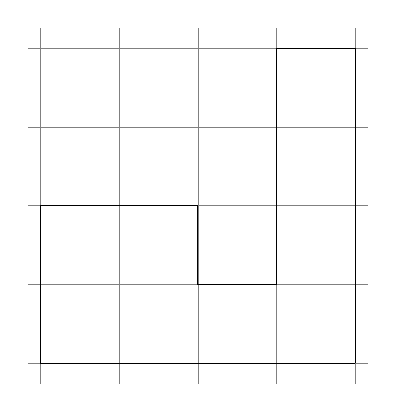
\begin{tikzpicture}[show background grid]
\draw[black] (0cm,0cm) -- (0cm,2cm);
\draw[black] (0cm,0cm) -- (0cm,2cm);
\draw[black] (0cm,2cm) -- (2cm,2cm);
\draw[black] (2cm,0.0cm) -- (0cm,0.0cm);
\draw[black] (2cm,2cm) -- (2cm,1cm);
\draw[black] (2cm,2cm) -- (2cm,1cm);
\draw[black] (2cm,1cm) -- (3cm,1cm);
\draw[black] (3cm,0.0cm) -- (2cm,0.0cm);
\draw[black] (3cm,1cm) -- (3cm,4cm);
\draw[black] (3cm,1cm) -- (3cm,4cm);
\draw[black] (3cm,4cm) -- (4cm,4cm);
\draw[black] (4cm,0.0cm) -- (3cm,0.0cm);
\draw[black] (4cm,4cm) -- (4cm,0.0cm);
\addvmargin{1mm}
\end{tikzpicture}
}
&
f)&\pbox{5cm}{
Berechne die Fläche von
\tikzstyle{background grid}=[draw, black!15,step=.5cm]
\noindent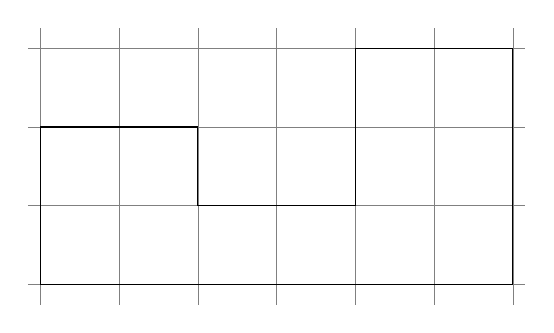
\begin{tikzpicture}[show background grid]
\draw[black] (0cm,0cm) -- (0cm,2cm);
\draw[black] (0cm,0cm) -- (0cm,2cm);
\draw[black] (0cm,2cm) -- (2cm,2cm);
\draw[black] (2cm,0.0cm) -- (0cm,0.0cm);
\draw[black] (2cm,2cm) -- (2cm,1cm);
\draw[black] (2cm,2cm) -- (2cm,1cm);
\draw[black] (2cm,1cm) -- (4cm,1cm);
\draw[black] (4cm,0.0cm) -- (2cm,0.0cm);
\draw[black] (4cm,1cm) -- (4cm,3cm);
\draw[black] (4cm,1cm) -- (4cm,3cm);
\draw[black] (4cm,3cm) -- (6cm,3cm);
\draw[black] (6cm,0.0cm) -- (4cm,0.0cm);
\draw[black] (6cm,3cm) -- (6cm,0.0cm);
\addvmargin{1mm}
\end{tikzpicture}
}
\\\hline
\end{xltabular}
\vspace{0.5cm}
\newpage
\rightline{Datum: 08.12.2023}
\centerline{{\large Lösungen Tägliche Übungen}} 
\vspace{0.5cm}

\begin{xltabular}{\textwidth}{|C{0.75cm}|X|C{0.75cm}|X|}
\arrayrulecolor{black}\hline
a)&\pbox{5cm}{
$A_1=2·1=2 cm^2$, $A_2=2·4=8 cm^2$, \\$A_3=2·3=6 cm^2$, $A= A_1+ A_2+ A_3=16 cm^2$\\
\tikzstyle{background grid}=[draw, black!15,step=.5cm]
\noindent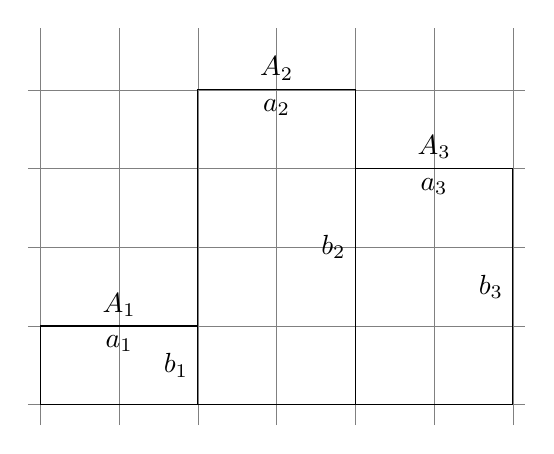
\begin{tikzpicture}[show background grid]
\draw[black] (0cm,0cm) rectangle (2cm,1cm);
\draw (1.0cm,1cm) node[below]{$a_1$}; 
\draw (2cm,0.5cm) node[left]{$b_1$}; 
\draw (1.0cm,1cm) node[above]{$A_1$}; 
\draw[black] (2cm,0cm) rectangle (4cm,4cm);
\draw (3.0cm,4cm) node[below]{$a_2$}; 
\draw (4cm,2.0cm) node[left]{$b_2$}; 
\draw (3.0cm,4cm) node[above]{$A_2$}; 
\draw[black] (4cm,0cm) rectangle (6cm,3cm);
\draw (5.0cm,3cm) node[below]{$a_3$}; 
\draw (6cm,1.5cm) node[left]{$b_3$}; 
\draw (5.0cm,3cm) node[above]{$A_3$}; 
\draw[black] (6cm,3cm) -- (6cm,0.0cm);
\addvmargin{1mm}
\end{tikzpicture}
}
&
b)&\pbox{5cm}{
$A_1=2·1=2 cm^2$, $A_2=2·4=8 cm^2$, \\$A_3=1·1=1 cm^2$, $A= A_1+ A_2+ A_3=11 cm^2$\\
\tikzstyle{background grid}=[draw, black!15,step=.5cm]
\noindent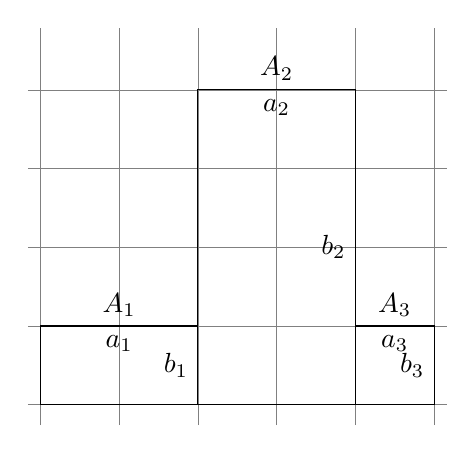
\begin{tikzpicture}[show background grid]
\draw[black] (0cm,0cm) rectangle (2cm,1cm);
\draw (1.0cm,1cm) node[below]{$a_1$}; 
\draw (2cm,0.5cm) node[left]{$b_1$}; 
\draw (1.0cm,1cm) node[above]{$A_1$}; 
\draw[black] (2cm,0cm) rectangle (4cm,4cm);
\draw (3.0cm,4cm) node[below]{$a_2$}; 
\draw (4cm,2.0cm) node[left]{$b_2$}; 
\draw (3.0cm,4cm) node[above]{$A_2$}; 
\draw[black] (4cm,0cm) rectangle (5cm,1cm);
\draw (4.5cm,1cm) node[below]{$a_3$}; 
\draw (5cm,0.5cm) node[left]{$b_3$}; 
\draw (4.5cm,1cm) node[above]{$A_3$}; 
\draw[black] (5cm,1cm) -- (5cm,0.0cm);
\addvmargin{1mm}
\end{tikzpicture}
}
\\\hline
c)&\pbox{5cm}{
$A_1=2·2=4 cm^2$, $A_2=2·3=6 cm^2$, \\$A_3=1·2=2 cm^2$, $A= A_1+ A_2+ A_3=12 cm^2$\\
\tikzstyle{background grid}=[draw, black!15,step=.5cm]
\noindent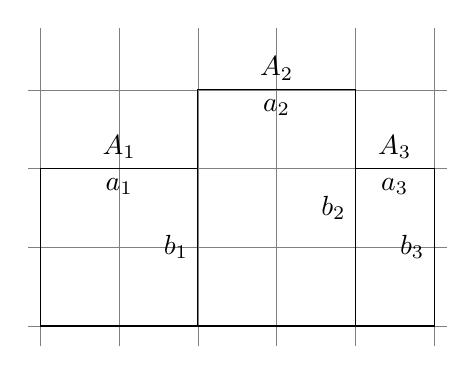
\begin{tikzpicture}[show background grid]
\draw[black] (0cm,0cm) rectangle (2cm,2cm);
\draw (1.0cm,2cm) node[below]{$a_1$}; 
\draw (2cm,1.0cm) node[left]{$b_1$}; 
\draw (1.0cm,2cm) node[above]{$A_1$}; 
\draw[black] (2cm,0cm) rectangle (4cm,3cm);
\draw (3.0cm,3cm) node[below]{$a_2$}; 
\draw (4cm,1.5cm) node[left]{$b_2$}; 
\draw (3.0cm,3cm) node[above]{$A_2$}; 
\draw[black] (4cm,0cm) rectangle (5cm,2cm);
\draw (4.5cm,2cm) node[below]{$a_3$}; 
\draw (5cm,1.0cm) node[left]{$b_3$}; 
\draw (4.5cm,2cm) node[above]{$A_3$}; 
\draw[black] (5cm,2cm) -- (5cm,0.0cm);
\addvmargin{1mm}
\end{tikzpicture}
}
&
d)&\pbox{5cm}{
$A_1=1·4=4 cm^2$, $A_2=1·3=3 cm^2$, \\$A_3=3·2=6 cm^2$, $A= A_1+ A_2+ A_3=13 cm^2$\\
\tikzstyle{background grid}=[draw, black!15,step=.5cm]
\noindent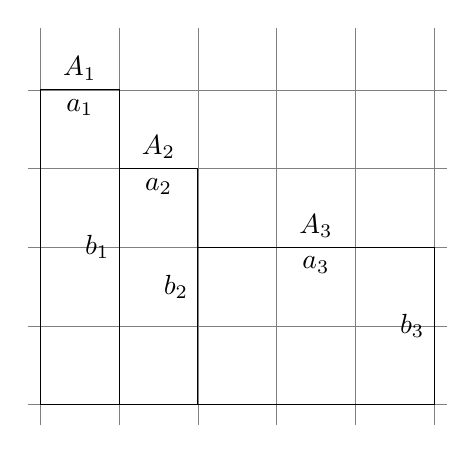
\begin{tikzpicture}[show background grid]
\draw[black] (0cm,0cm) rectangle (1cm,4cm);
\draw (0.5cm,4cm) node[below]{$a_1$}; 
\draw (1cm,2.0cm) node[left]{$b_1$}; 
\draw (0.5cm,4cm) node[above]{$A_1$}; 
\draw[black] (1cm,0cm) rectangle (2cm,3cm);
\draw (1.5cm,3cm) node[below]{$a_2$}; 
\draw (2cm,1.5cm) node[left]{$b_2$}; 
\draw (1.5cm,3cm) node[above]{$A_2$}; 
\draw[black] (2cm,0cm) rectangle (5cm,2cm);
\draw (3.5cm,2cm) node[below]{$a_3$}; 
\draw (5cm,1.0cm) node[left]{$b_3$}; 
\draw (3.5cm,2cm) node[above]{$A_3$}; 
\draw[black] (5cm,2cm) -- (5cm,0.0cm);
\addvmargin{1mm}
\end{tikzpicture}
}
\\\hline
e)&\pbox{5cm}{
$A_1=2·2=4 cm^2$, $A_2=1·1=1 cm^2$, \\$A_3=1·4=4 cm^2$, $A= A_1+ A_2+ A_3=9 cm^2$\\
\tikzstyle{background grid}=[draw, black!15,step=.5cm]
\noindent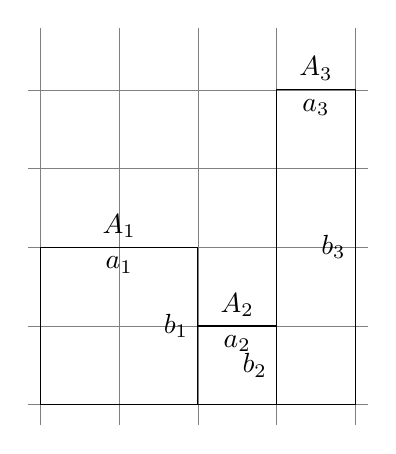
\begin{tikzpicture}[show background grid]
\draw[black] (0cm,0cm) rectangle (2cm,2cm);
\draw (1.0cm,2cm) node[below]{$a_1$}; 
\draw (2cm,1.0cm) node[left]{$b_1$}; 
\draw (1.0cm,2cm) node[above]{$A_1$}; 
\draw[black] (2cm,0cm) rectangle (3cm,1cm);
\draw (2.5cm,1cm) node[below]{$a_2$}; 
\draw (3cm,0.5cm) node[left]{$b_2$}; 
\draw (2.5cm,1cm) node[above]{$A_2$}; 
\draw[black] (3cm,0cm) rectangle (4cm,4cm);
\draw (3.5cm,4cm) node[below]{$a_3$}; 
\draw (4cm,2.0cm) node[left]{$b_3$}; 
\draw (3.5cm,4cm) node[above]{$A_3$}; 
\draw[black] (4cm,4cm) -- (4cm,0.0cm);
\addvmargin{1mm}
\end{tikzpicture}
}
&
f)&\pbox{5cm}{
$A_1=2·2=4 cm^2$, $A_2=2·1=2 cm^2$, \\$A_3=2·3=6 cm^2$, $A= A_1+ A_2+ A_3=12 cm^2$\\
\tikzstyle{background grid}=[draw, black!15,step=.5cm]
\noindent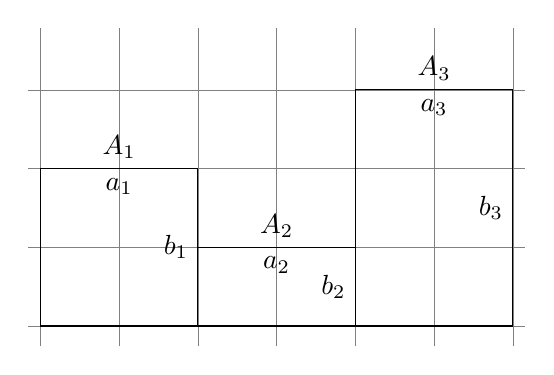
\begin{tikzpicture}[show background grid]
\draw[black] (0cm,0cm) rectangle (2cm,2cm);
\draw (1.0cm,2cm) node[below]{$a_1$}; 
\draw (2cm,1.0cm) node[left]{$b_1$}; 
\draw (1.0cm,2cm) node[above]{$A_1$}; 
\draw[black] (2cm,0cm) rectangle (4cm,1cm);
\draw (3.0cm,1cm) node[below]{$a_2$}; 
\draw (4cm,0.5cm) node[left]{$b_2$}; 
\draw (3.0cm,1cm) node[above]{$A_2$}; 
\draw[black] (4cm,0cm) rectangle (6cm,3cm);
\draw (5.0cm,3cm) node[below]{$a_3$}; 
\draw (6cm,1.5cm) node[left]{$b_3$}; 
\draw (5.0cm,3cm) node[above]{$A_3$}; 
\draw[black] (6cm,3cm) -- (6cm,0.0cm);
\addvmargin{1mm}
\end{tikzpicture}
}
\\\hline
\end{xltabular}
\vspace{0.5cm}
\end{document}